\chapter{Sjabloon DMP}
\label{ap:dmp}
Onderstaand sjabloon voor het maken van een DMP kan je gebruiken voor je projecten. Je mag dit uiteraard ook aanpassen indien nodig. Dit sjabloon is verkregen van de \href{https://libguides.ru.nl/datamanagement/dm}{\textsf{universiteitsbibliotheek van de Radboud Universiteit}}. Via die link vind je ook nog wat extra informatie en voorbeelden. Het saxion heeft ook informatie over een DMP, dat kan je vinden op de site van de \href{https://srs.saxion.nl/}{\textsf{Saxion Research Services}}. Het DMP-sjabloon van het Saxion is erg uitgebreid en vooral geschikt voor grote onderzoeken, vandaar dat in dit dictaat de voorkeur naar het kortere sjabloon van de RU gaat. 

Gebaseerd op een werk van de Universiteitsbibliotheek Nijmegen op \href{http://ru.nl.libguides.com}{\textsf{http://ru.nl.libguides.com}}
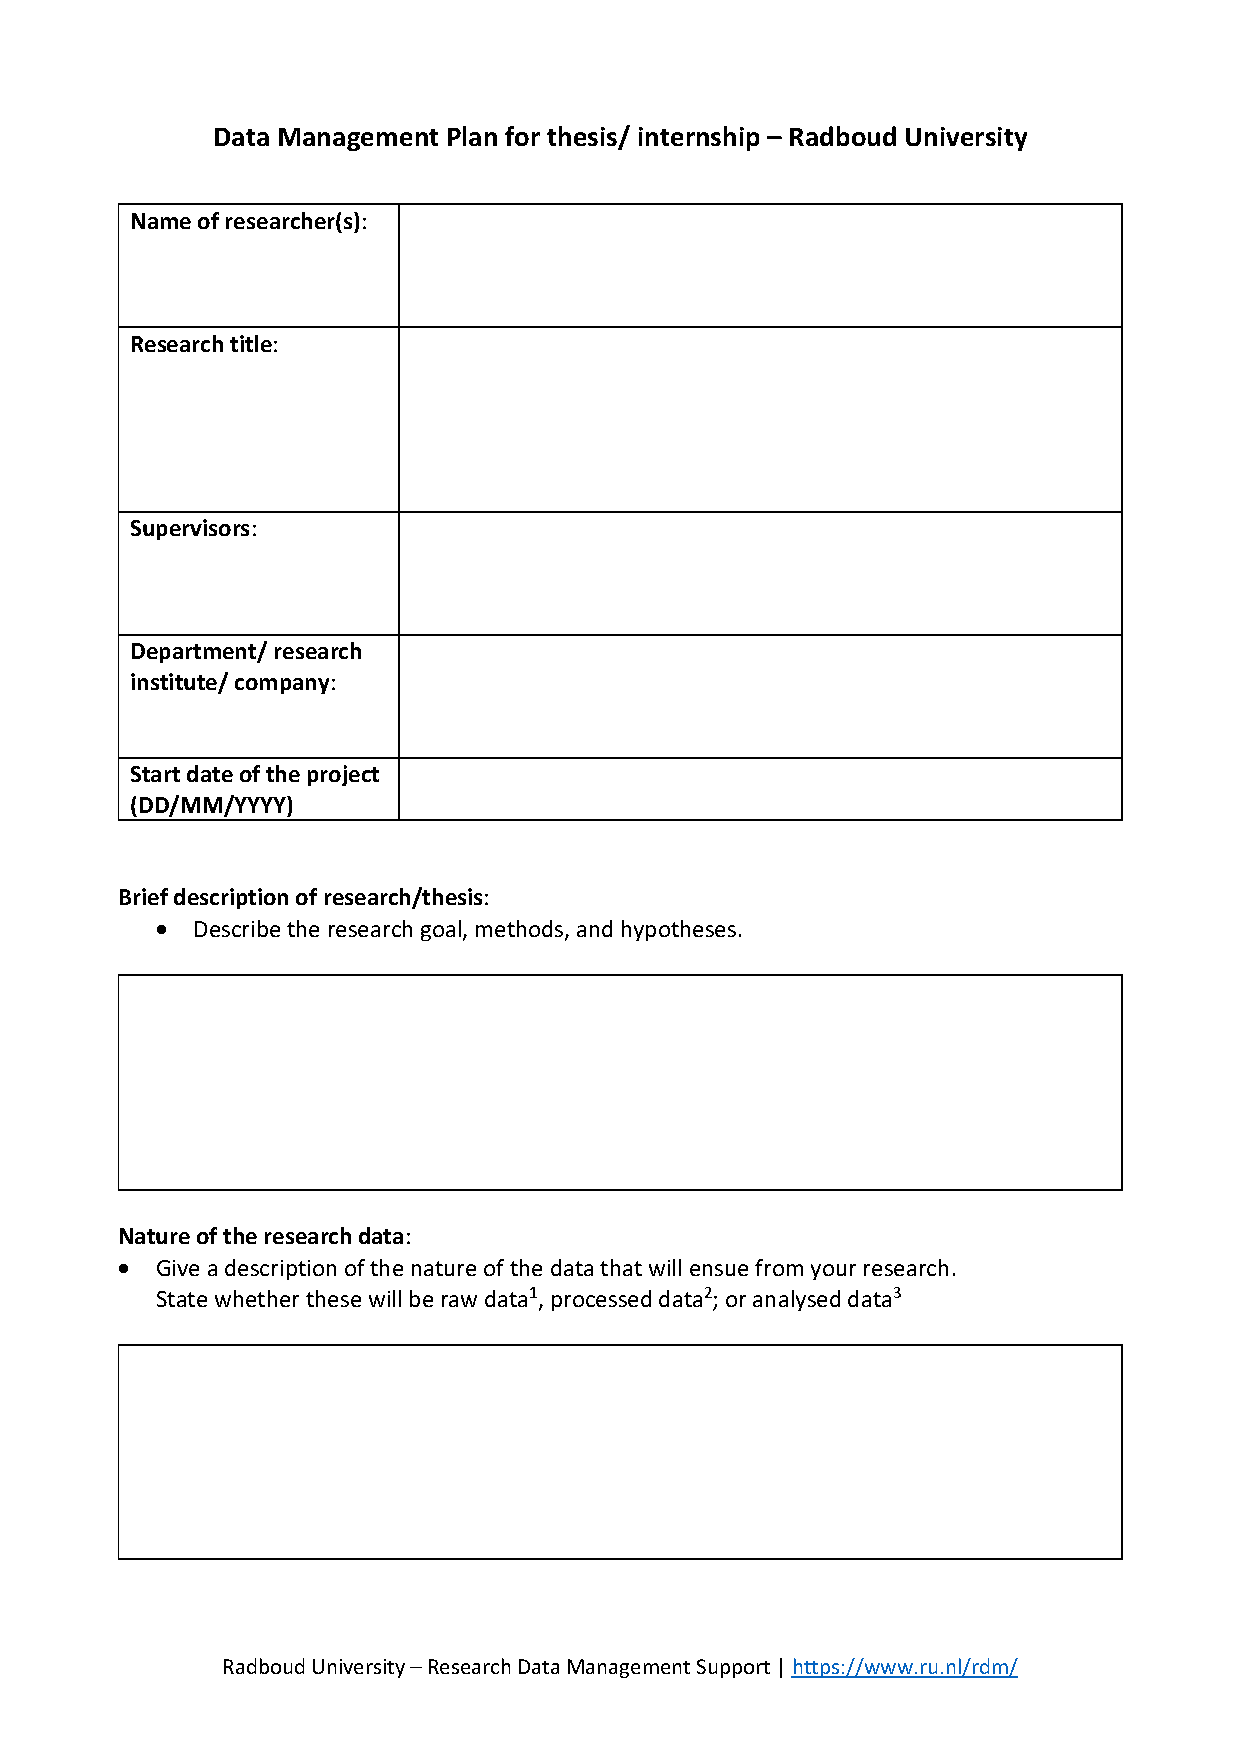
\includepdf[pages=-, nup=2x2]{img/dmp.pdf}
